\documentclass[border=2pt]{standalone}
\usepackage{tkz-euclide}
\usetkzobj{all}
\begin{document}

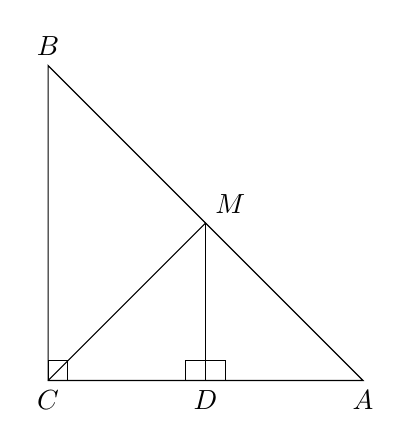
\begin{tikzpicture}
\coordinate (B) at (0,4);
\coordinate (A) at (4,0);
\coordinate (C) at (0,0);
\coordinate (D) at (2,0);
\coordinate (M) at (2,2);
\draw (A)node[below]{$A$}--(B)node[above]{$B$}--(C)node[below]{$C$}--cycle;
\draw(M)node[above right]{$M$}--(D)node[below]{$D$};
\draw(M)--(D);
\draw(M)--(C);
\tkzMarkRightAngle(B,C,A)
\tkzMarkRightAngle(A,D,M)
\tkzMarkRightAngle(C,D,M)
\end{tikzpicture}
\end{document}